\documentclass[10pt,a4paper]{article}
\usepackage[utf8]{inputenc}
\usepackage[fleqn]{amsmath}
\usepackage{amssymb}
\usepackage{float}
\usepackage{enumerate}
\usepackage{graphicx}
\usepackage{tikz}
\usepackage{parskip}
\usepackage{listings}
\usepackage[left=2cm,right=2cm,top=2cm,bottom=2cm]{geometry}
\title{FYP Progress Meeting}
\author{Thomas Carroll}
\date{2021-03-30}
\begin{document}
\maketitle{}
\section{Summary of Progress}
The concept of the project was initially to enable users to intuitively work out
how to navigate a set of parameters to draw art to the screen.

The art is based on pen-plotter work by artist \emph{Darrell Viner} a relatively
unknown artist but one of the first British computer artists. His work is held
in the Henry Moore and V\&A museums.

Exploring multiple parameters is equivalent to exploring a multi-dimensional
feature space so information was gathered on how existing solutions achieved
this, most seemed to include dimensional reduction in some sense or another.
Some chose to visualise subspaces and others chose to show slices of the space.
These were both interesting but the slicing approach made more sense for the
purpose of this project because it didn't remove any part of the feature space,
this can be seen as allowing the user the change any parameter at will.

Control schemes were considered too, the idea being that a user should be able
to understand how to operate the program in the context of home use. For this
reason custom controllers were out of the question despite being more suited
(e.g. knobs that controlled each parameter).

Generating the art also posed challenges, this involved a review of Viner's work
to see what techniques he may have used and to translate them into modern
computing (his work was completed in \verb|FORTRAN|). 

Part of this was conceiving of a way to generate a `landscape' that could be
used to inform the generation of the art. This involved creating tools that can
be combined to generate points that conform to a coherent geometry. An example
of this would be using Perlin noise in combination with an approximate rounding
function using additive synthesis to create a `semi-quantised' noise. Using
Perlin noise makes sense here because of it's ability to be `natural' looking
but also procedural based on a set of parameters and a seed, allowing for
reproducibility of states.

\begin{figure}[H]
\centering
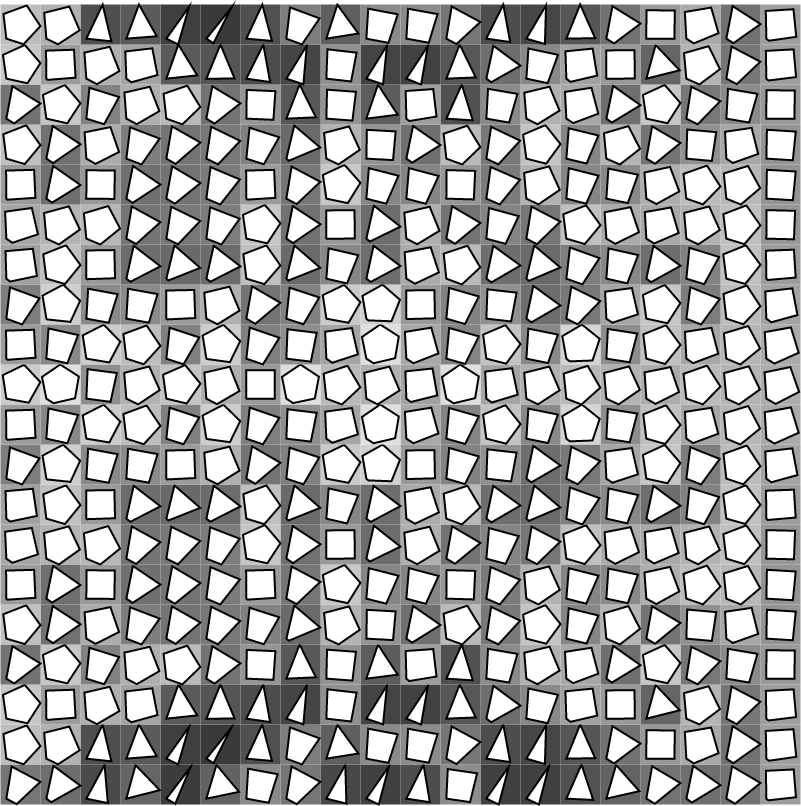
\includegraphics[width=.3\textwidth]{noisewithPolygons}
\hspace{0.2cm}
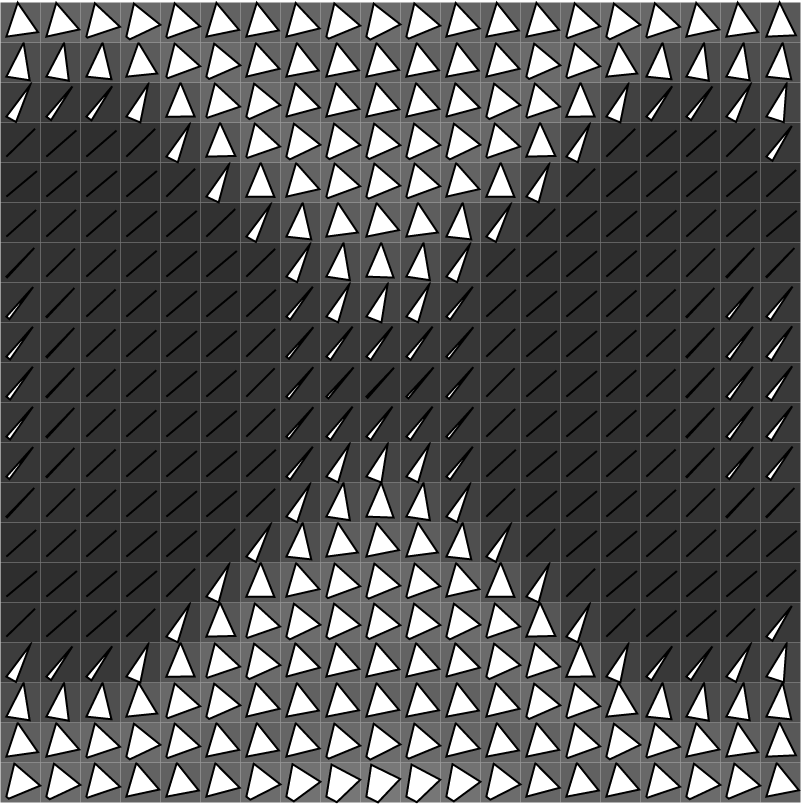
\includegraphics[width=.3\textwidth]{noisewithPolygons1term}
\end{figure}

Also to help with navigation a concept for generating musical intervals (ratios
of pitches) was developed, this has yet to be fully implemented but a demo shows
that it may be useful in helping users locate themselves within the set of
parameters they are able to control. Further this would add an element to the
art that is `non-Viner', so to speak, and perhaps makes the work feel more `in
dialogue' with the work than directly copying, as well as making it more
engaging for users.

A system was devised to recall previous states of the visuals using a tree data
structure, whilst not complete it allows for saving and loading in histories as
json files and a visualisation of the tree that saved the states you are in.
This allows users to recall any state from a session and save and share states
with others. This system saves the state every 100 frames and if the user wants
to access somewhere between those states it can linearly interpolate between
them.

\begin{figure}[H]
\centering
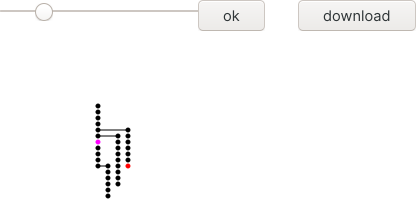
\includegraphics[width=.7\textwidth]{tree}
\caption{Current interface: (subject to change), red is current position and pink
is `cursor' to recall position when `ok' is pressed. Ideally you would just
click on the `map'}
\end{figure}

\section{Todo}
The history system needs to be completed first, and is being worked on
currently, this would allow work to be started on general UI polishing.

The user interface needs to have ways to change parameters and explain key
bindings to the user. Ultimately this would ideally be able to be hidden totally
so that the user can see only the grid.

There should be some way to save images from the screen to the user's computer
too, perhaps as a stretch to allow videos to be generated, but the tools
available to do this would need to be explored more. 

I would also like to perhaps look at a method to show a large `map' that shows
everything a user has seen in a session, perhaps only in one branch of the tree
history. This would need to be considered a bit more.

The music part needs to be worked on, I am collecting recordings to try and
build some samples for this. All of the component parts are there, all that
needs to be done is integration and implementation of the generative music part.

Overall the graphics themselves are almost there but could do with more polish,
it's a bit indeterminate but things like creating more flexible offsets for each
point's calculation to allow for a less constrained set of images. 

Perhaps also this could be tested with some users remotely to see if the goals
of understanding how users can control the application work, but this might not
fit to formal user testing methods as it's an art project.
\end{document}
